\documentclass[fontset=none]{ctexart}

\usepackage[T1]{fontenc}
\usepackage{fontspec}
\setCJKmainfont{SimSun}
% Latin Modern
\renewcommand*\ttdefault{txtt} % 改等宽字体

\setcounter{tocdepth}{5}
\setcounter{secnumdepth}{5}
% -1 part
% 0 chapter
% 1 section
% 2 subsection
% 3 subsubsection
% 4 paragraph
% 5 subparagraph

\usepackage{cite}
\usepackage{geometry}
\geometry{a4paper,scale=0.7}

\usepackage{algorithm}  
\usepackage{algorithmicx}  
\usepackage{algpseudocode}
\makeatletter
\newenvironment{breakablealgorithm}
  {% \begin{breakablealgorithm}
   \begin{center}
     \refstepcounter{algorithm}% New algorithm
     \hrule height.8pt depth0pt \kern2pt% \@fs@pre for \@fs@ruled
     \renewcommand{\caption}[2][\relax]{% Make a new \caption
       {\raggedright\textbf{\ALG@name~\thealgorithm} ##2\par}%
       \ifx\relax##1\relax % #1 is \relax
         \addcontentsline{loa}{algorithm}{\protect\numberline{\thealgorithm}##2}%
       \else % #1 is not \relax
         \addcontentsline{loa}{algorithm}{\protect\numberline{\thealgorithm}##1}%
       \fi
       \kern2pt\hrule\kern2pt
     }
  }{% \end{breakablealgorithm}
     \kern2pt\hrule\relax% \@fs@post for \@fs@ruled
   \end{center}
  }
\makeatother

\usepackage{amsmath}
\usepackage{amssymb}
\usepackage{graphicx}
\usepackage{subfigure}
\usepackage{changepage}
\usepackage{multirow}
\usepackage{url}

\usepackage{amsthm}
\newtheorem{theorem}{Theorem}[section]
\newtheorem{lemma}[theorem]{Lemma}
\newtheorem{proposition}[theorem]{Proposition}
\newtheorem{corollary}[theorem]{Corollary}
% \newtheorem{remark}{Remark}[section]
\newtheorem{example}{Example}[section]
\newenvironment{solution}{\begin{proof}[Solution]}{\end{proof}}
\theoremstyle{definition}
\newtheorem{definition}{Definition}[section]
\theoremstyle{remark}
\newtheorem*{remark}{Remark}

\usepackage[colorlinks, linkcolor=black, citecolor=blue, bookmarksnumbered]{hyperref}
% \hypersetup{
% 	colorlinks=true,
% 	linkcolor=cyan,
% 	filecolor=blue,      
% 	urlcolor=red,
% 	citecolor=green,
% }

\usepackage{fancyhdr}
\pagestyle{fancy}
\renewcommand{\sectionmark}[1]{\markright{\thesection\ #1}}
\fancyhf{}
\cfoot{\thepage}
\lhead{\rightmark}
% \rightmark 当前的节名
% \leftmark 当前的章名
% \(l/c/r)head{}, \(l/c/r)foot{}
\renewcommand{\headrulewidth}{0.4pt}
\renewcommand{\footrulewidth}{0pt}

\renewcommand\refname{References}
\renewcommand\contentsname{Content}
\renewcommand\figurename{Figure}

\begin{document}

\begin{titlepage}
    \begin{center}
        \vspace*{1cm}
            
        \Huge
        \textbf{Implementation Of A TTE System}
            
        \vspace{0.5cm}
        \LARGE
        First Report\\
            
        \vspace{1.5cm}
            
        \textbf{11812804}  董\quad 正\\
        \textbf{11813225}  王宇辰\\
        \textbf{11811305}  崔俞崧\\

        \vspace{0.5cm}
        Supervisior: 宋轩
            
        \vfill
            
        
\includegraphics[width=\textwidth]{images/sustc.png}
            
        \vspace{0.2cm}
            
        \Large
        Department of Computer Science and Engineering\\
        \vspace{0.5cm}
        Apr. 2021
            
    \end{center}
\end{titlepage}

\tableofcontents

\clearpage
\section{Preliminaries}
\subsection{Review}
\subsubsection{TTE}
\textbf{Travel Time Estimation (TTE)} is one of the most important researching topic in the traffic forecasting field. 
Estimating the travel time of any path in a city is of great importance to traffic monitoring, route planning, ridesharing, taxi dispatching, etc.
On Sep. 2020, DeepMind published a blog named \textit{Traffic prediction with advanced Graph Neural Networks}. 
This blog briefly described the whole industrial structure of estimated times of arrival (ETAs) techniques applied in Google Map but did not given any detailed implementation or any code.
Our work is based on the model structure of TTE proposed in the blog.
\begin{figure}[htb]
    \centering
    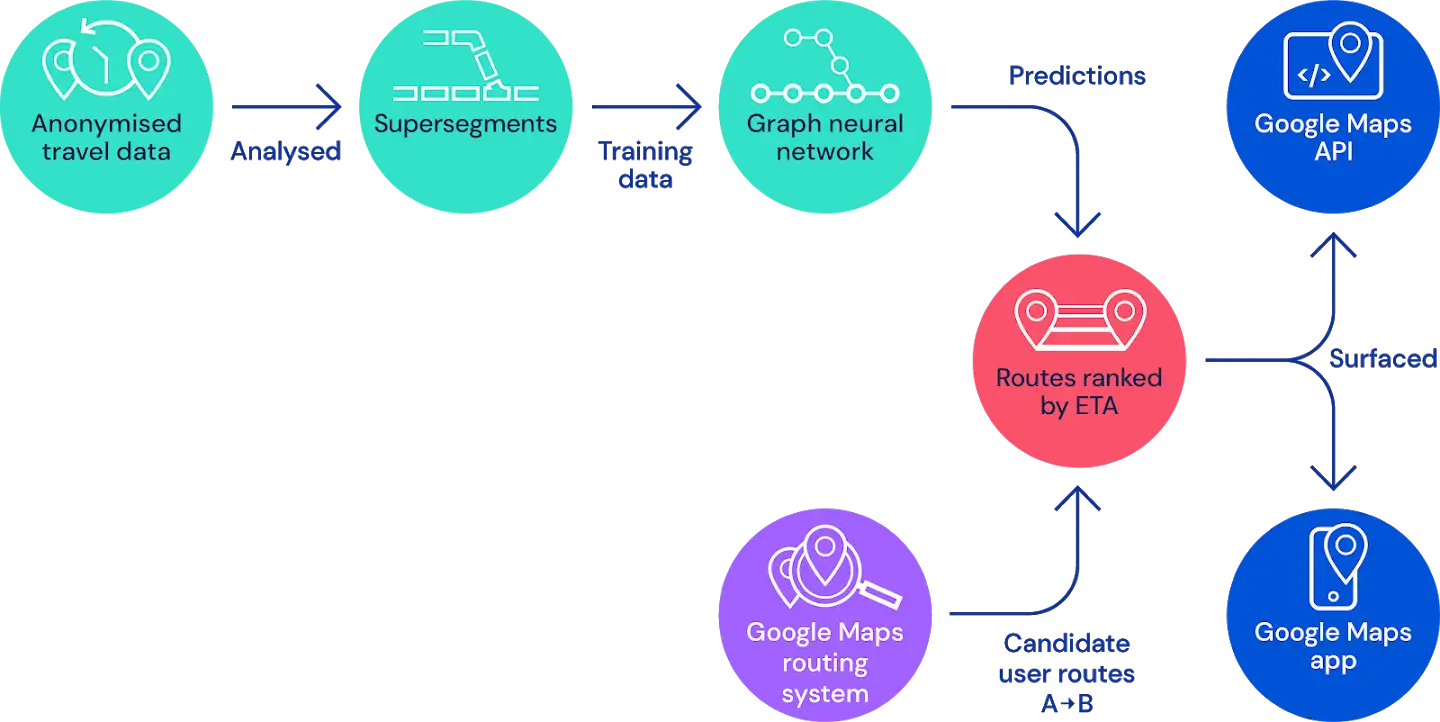
\includegraphics[width=0.9\textwidth]{images/architecture.png}
    \caption{Architecture}
    \label{fig1}
\end{figure}

\subsubsection{Goal}
Our ultimate goal (tentative) is to implement the industrial structure and apply it to the open source databases in China, then compare the performance with the state-of-the-art structures and find its application value.
This semester, we will implement a TTE system base on the work we done in the last term, combining \textit{supersegment} and \textit{DeepTTE}.
We will try to work out an interactive application with graphical user interface. 

\subsection{Introduction}
In the last stage, we have processed some open source data. And we got deep in the code of \textit{DeepTTE} and researched on a new concept
called \textbf{Travel Time Index (TTI)}. In addition, we proposed a new computing process of \textit{Supersegment} and gave a simple demo.

Breifly, we will state our work in this report as
\begin{itemize}
    \item xxx by 王宇辰
    \item xxx by 崔俞崧
    \item Code implementation of \textit{Supersegment} by 董正
\end{itemize}

\clearpage
\section{xxx}

\clearpage
\section{xxx}

\clearpage
\section{Code Implementation of Supersegment}
\subsection{Dataset}
\begin{itemize}
    \item Data source: Didi Chuxing GAIA Intiative
    \item Region: Chengdu
    \item Time: 2018-10-01 to 2018-12-01
    \item Content:
        \begin{itemize}
            \item GPS track of taxis with timestamps
            \item Coordinate of road and district boundaries
            \item TTI and average speed of districts
        \end{itemize}
\end{itemize}
\begin{figure}[htb]
  \centering
  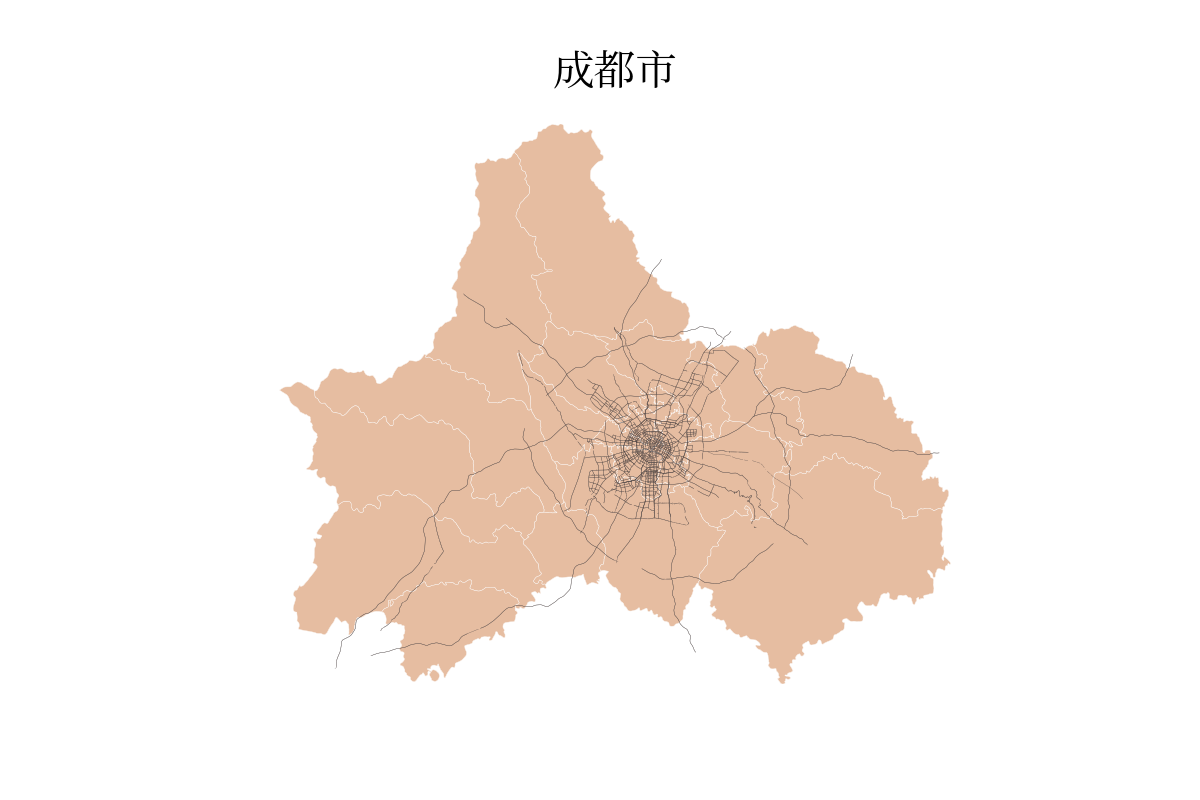
\includegraphics[width=\textwidth]{images/成都市.png}
  \caption{Cheng Du}
  \label{fig: chengdu}
\end{figure}

\subsection{Model Design}
In this section, I will propose a model to compute Supersegments.
At the very first, I need to ensure that I will base on \textbf{speed} to do the division.
There is a three-step approach of my design:
\begin{enumerate}
    \item Locate GPS coordinates of taxis into corresponding roads
    \item Use the timestamps to calculate average speed and regard it as the instantaneous speed of midpoint
    \item Apply clustering algorithm to these midpoints
    \item Intersect road and clusters to get segments
\end{enumerate}

First, since we know the boundaries of the roads, we can determine the coordinate is on which road.
After that, we draw the GPS points on the road. Because we know the timestamp of each point, we can 
calculate the average speed of two adjacent points and just consider it as the speed of their midpoint.
Note that the closer the points are, the closer the average speed is to the actual instantaneous speed.
So the best way is to select adjacent points if our data is abundant.
\begin{figure}[htb]
  \centering
  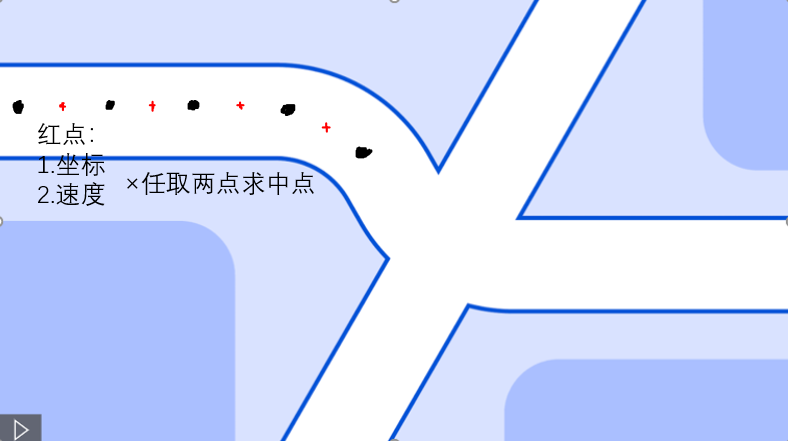
\includegraphics[width=0.9\textwidth]{images/midpoints.png}
  \caption{Find the midpoints}
  \label{fig: midpoint}
\end{figure}

Next step is to apply clustering algorithm like \textit{K-Means} or \textit{MeanShift} to find a certain number of clusters
of the midpoints.
Every midpoint has three features:
\begin{itemize}
  \item longitude
  \item latitude
  \item speed
\end{itemize}

So actually this is a three-dimension clustering, but the result we need is two-dimensional, which means
we need to balance the weight of these features carefully to get a correct partition.
\begin{figure}[h]
  \centering
  \subfigure[Clusters] {
    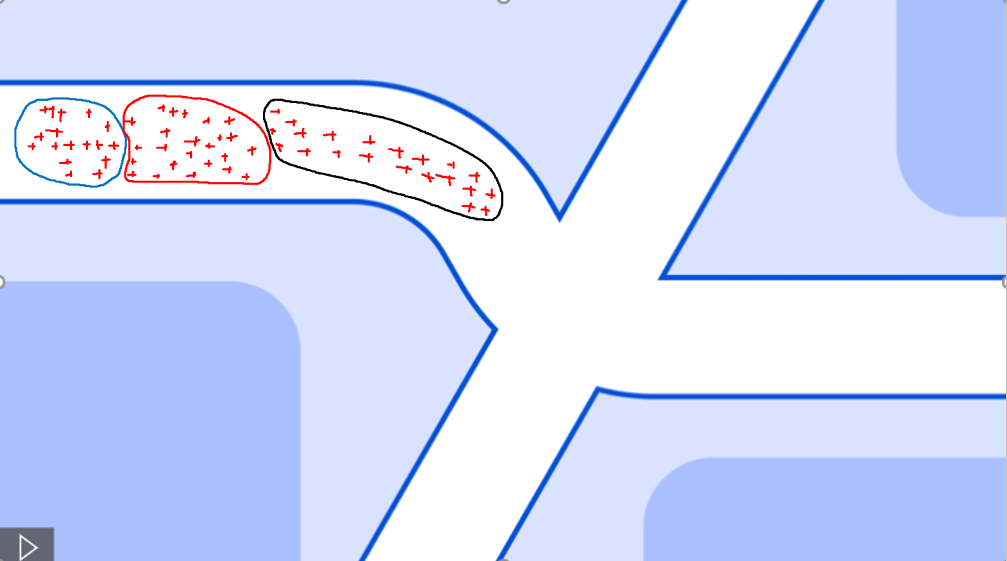
\includegraphics[width=0.45\textwidth]{images/cluster.png}
  }
  \quad
  \subfigure[K-Means Example] {
    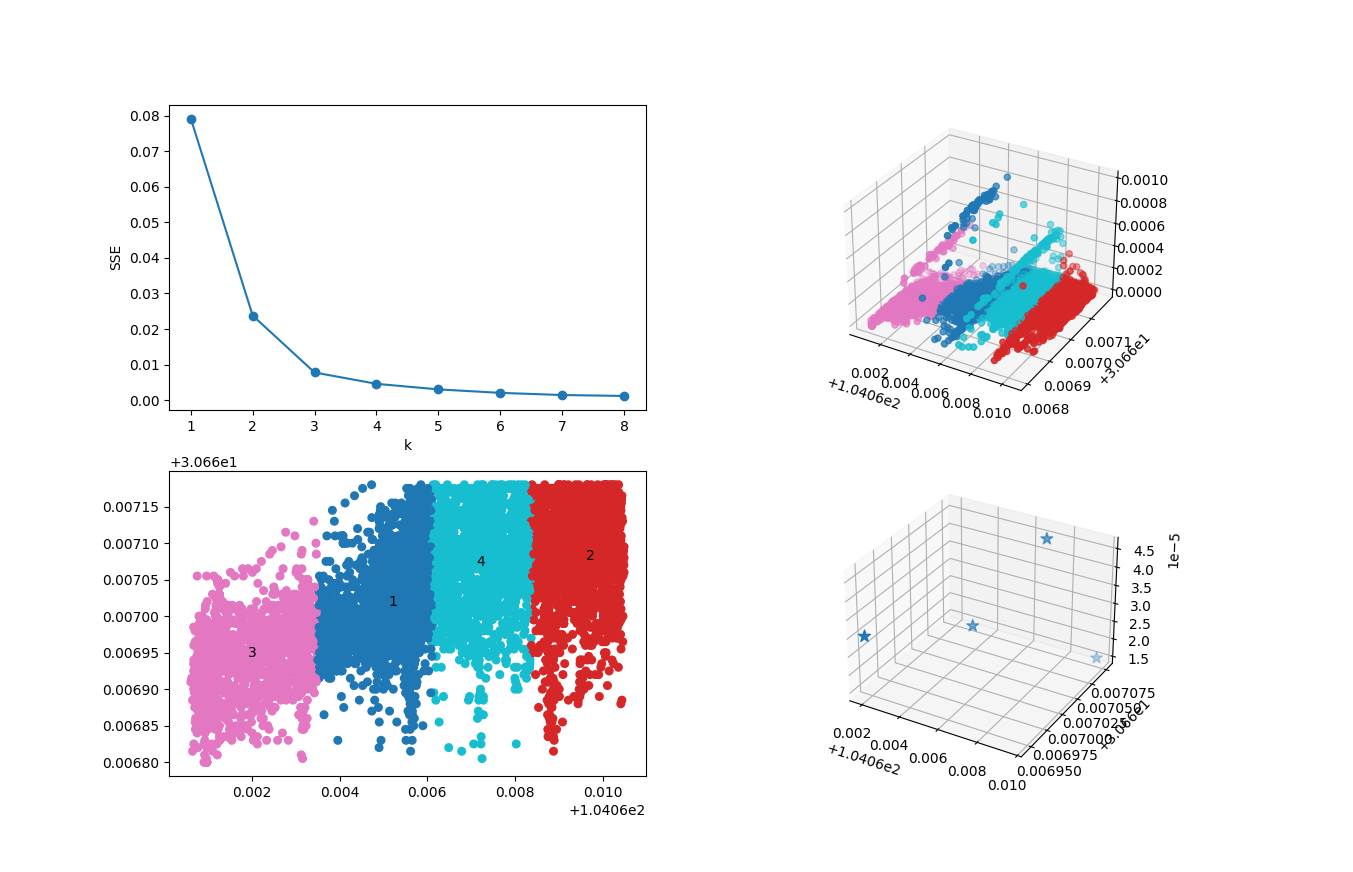
\includegraphics[width=0.45\textwidth]{images/5000辆车kmeans.png}
  }
\end{figure}

Finally, compute the convex hull of each cluster and find its intersection with the roads.
Therefore, we have partitioned the roads into several segments.

\clearpage
\subsection{Code Implementation}
\subsubsection{Map Matching}
The first step is to locate GPS point into roads. This problem is called \textbf{Map Matching}.

In our dataset, a road is represented as a line, however, it should be an area in real world.
Besides, it is hard to match a point to a 2-D line. Therefore, we need to convert a road to an area in advance.

Use method \texttt{buffer()} in \textit{shapely} package.
\begin{figure}[htb]
  \centering
  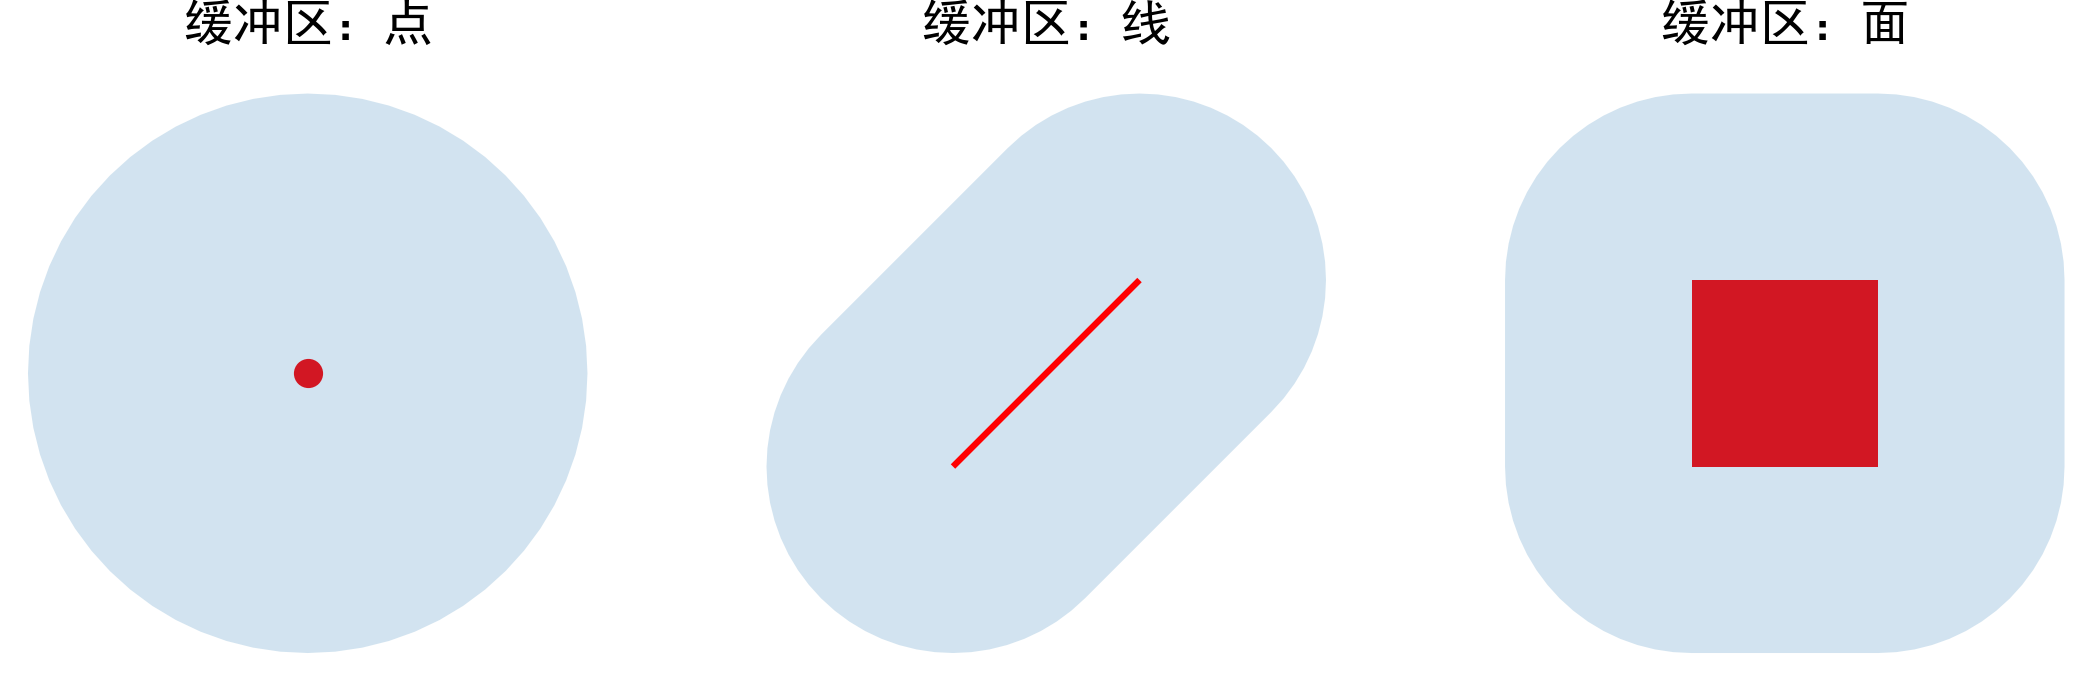
\includegraphics[width=0.9\textwidth]{images/buffer_example.png}
  \caption{\texttt{buffer()}}
  \label{fig: buffer}
\end{figure}

The \texttt{buffer()} method will convert a \texttt{Line} to a \texttt{Polygon}.

Take 羊市街 + 西玉龙街 and the tracks of 10,000 taxis as an example. Actually there are three roads.
Apply this function to the roads and we will get
\begin{figure}[htb]
  \centering
  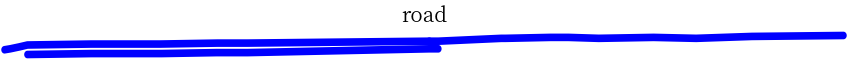
\includegraphics[width=0.9\textwidth]{images/roads.png}
  \caption{Buffered Roads}
  \label{fig: roads}
\end{figure}

Secondly, filter the data. Use method \texttt{geopandas.GeoSeries.total\_bounds} to get the bottom left corner
and the upper right corner of these roads, then screen out the points which are not in the rectangle area.

Finally, for each point, find which road it in by \texttt{contains()} method in \textit{shapely} package.
\begin{figure}[htb]
  \centering
  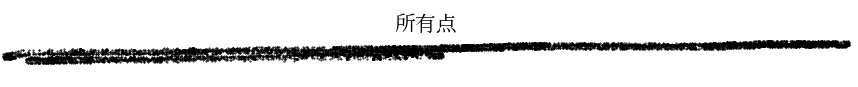
\includegraphics[width=0.9\textwidth]{images/all_points_new.png}
  \caption{Matched Points}
  \label{fig: points}
\end{figure}

\subsubsection{Calculate Midpoints}
In this step, we calculate the coordinate and speed of the midpoints.

First thing to notice is that we should use the point in the same track, otherwise the timestamps are not
continuous, resulting in a wrong speed.

In addtion, after working out the midpoints, we need to match these points again into the roads because
there are some arc-shaped roads so that the midpoints may be in the interior of the arc.

\begin{figure}[htb]
  \centering
  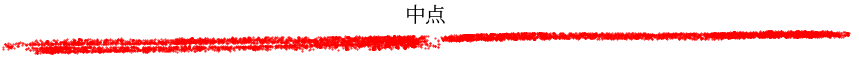
\includegraphics[width=0.9\textwidth]{images/midpoints_new.png}
  \caption{Midpoints}
  \label{fig: midpoints}
\end{figure}

\clearpage
\subsubsection{Clustering}
In this step, we use \textit{KMeans} or \textit{MeanShift} in \textit{sklearn} package.
\begin{figure}[htb]
  \centering
  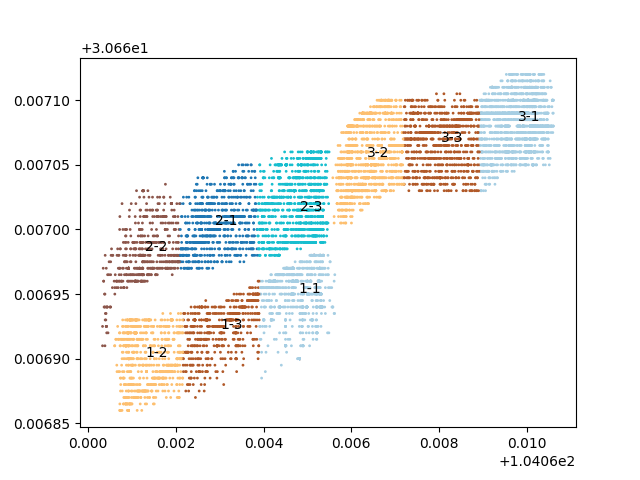
\includegraphics[width=0.9\textwidth]{images/kmeans_new.png}
  \caption{KMeans}
  \label{fig: kmeans}
\end{figure}
\clearpage
\begin{figure}[htb]
  \centering
  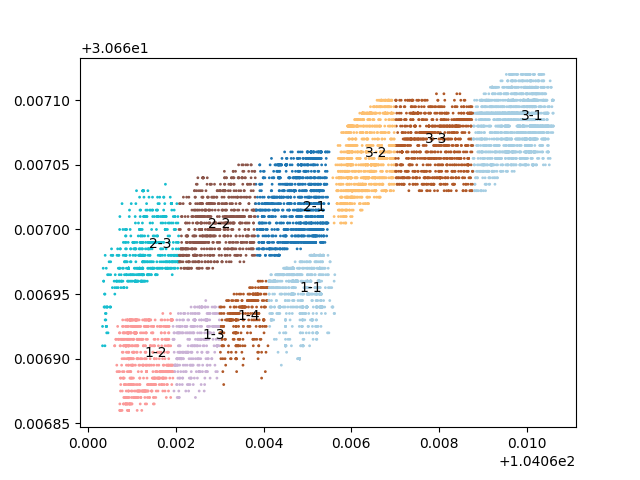
\includegraphics[width=0.9\textwidth]{images/meanshift.png}
  \caption{MeanShift}
  \label{fig: meanshift}
\end{figure}

\subsubsection{Intersection}
The last step is to compute the intersection of the clusters and the roads.

First we need to calculate the convex hull of the clusters, because we cannot use the intersection
of line and points. Use \texttt{geopandas.GeoSeries.convex\_hull} to compute the convex hull of the
clusters. Then use \texttt{intersection()} method in \textit{shapely} package to get the intersection.
\begin{figure}[htb]
  \centering
  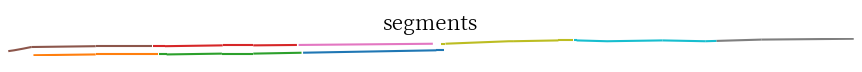
\includegraphics[width=0.9\textwidth]{images/segments.png}
  \caption{Segments}
  \label{fig: segments}
\end{figure}

% \clearpage
% \phantomsection
% \addcontentsline{toc}{section}{References}
% \bibliographystyle{ieeetr}
% \bibliography{references}

\end{document}